\section{Discussions}
The RAG pipeline has significantly improved the performance of the LLM by grounding responses in relevant external context. However, the results are far from perfect and several challenges and unresolved issues remain that need to be addressed for better performance.

The success of RAG heavily depends on the relevance and quality of the retrieved documents. If the retrieval mechanism brings back irrelevant or low-quality documents, the generation process can be adversely affected, leading to inaccurate or irrelevant responses. It is crucial to improve retrieval algorithms to better assess and rank document relevance for enhancing RAG performance.

RAG models sometimes struggle with ambiguous or highly diverse queries that do not have a clear, single relevant document. Enhancing RAG’s ability to handle such queries is necessary for providing more accurate responses. As part of an experiment conducted\footnote{\url{https://github.com/winterForestStump/thesis/blob/main/notebooks/question_rag_x_phi3_experiment.ipynb}}, the question "What is the company's total outstanding debt, how is the debt structured, and what are the interest rates?" was re-asked to the RAG system for about 10 companies (the same companies used in the main experiments), and since the question actually consists of three relatively independent sub-questions "What is the company's total outstanding debt?", "How is the company's debt structured?", "What are the interest rates for company's debt?", each sub-question was also asked to the system. The results obtained were evaluated using the same methodology as the main experiments (described in detail in the Experiments and Results section). The average results obtained for each metric and question are summarized in the heatmap\footnote{\url{https://github.com/winterForestStump/thesis/blob/main/evaluation/question_bge-reranker_x_phi3-4k/question_partition__eval_results.ipynb}} on \autoref{fig:question_partition_heatmap}:
\begin{figure}[h!]
\centering
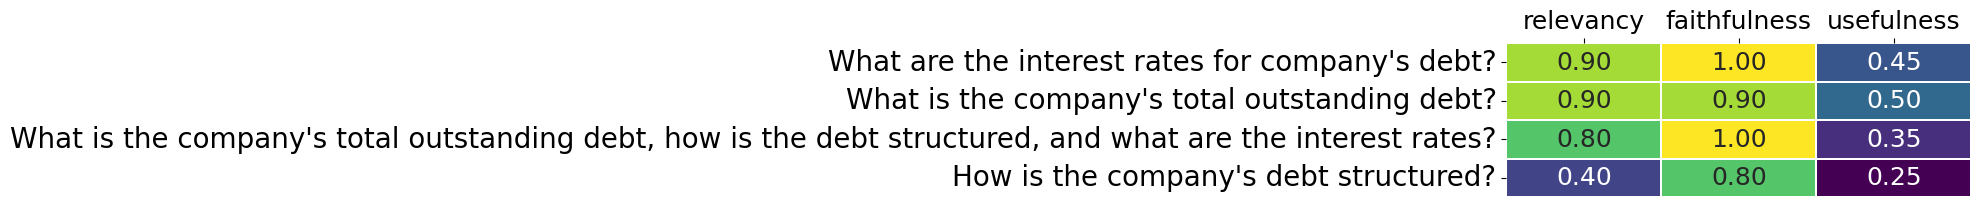
\includegraphics[width=1\textwidth]{Figures/question_partition_heatmap.png}
\caption{The heatmap for the question partition experiment}
\label{fig:question_partition_heatmap}
\end{figure}
The results show that two of the three sub-questions have mean higher than that of the main question. This is especially true for 'relevancy' and 'usefulness'. It can be assumed that the debt structure question is problematic for the system and affects more the decrease of the metrics for the main question. However, this issue requires further investigation.

Retrieval granularity denotes the retrieval unit in which the corpus is indexed, such as documents, passages, or tokens. For RAG, the choice of retrieval granularity can significantly impact performance. Larger chunks capture more context but generate more noise, requiring longer processing time and higher costs. Smaller chunks, while less noisy, may not fully convey the necessary context. Optimizing a recursive splits and sliding window method can help balance semantic completeness and context length. Furthermore, document chunking based on structure instead of paragraphs can improve the quality of RAG's outputs \cite{Yepes.5Feb2024}.

One of the primary limitations of current RAG architectures is their inability to integrate content from previous conversation turns. Each response is generated based solely on the immediate input query, without considering the dialogue history. This limitation can result in a lack of continuity and coherence, as the model cannot reference or build upon previous turns. The model might provide inconsistent responses since it doesn't have the context of earlier interactions to ensure alignment. Effective incorporation of conversation history is essential for more human-like interactions.

The feature encoder always plays a vital role in natural language processing tasks. Better embedding models are more likely to fetch similarities across contexts and help identify highly relevant context \cite{Dong.28May2024}. Various approaches to embeddings can significantly impact the performance of RAG systems. Although we did not conduct experiments with different chunking strategies and embedding models, it is evident that more advanced approaches could yield substantially different results. For instance, an element-based chunking strategy improved performance in state-of-the-art Q\&A tasks on the FinanceBench Questions dataset \cite{Yepes.5Feb2024}. This improvement was achieved by adopting a better chunking strategy for processing documents, compared to baseline chunking strategies using fixed chunk sizes of 128, 256, and 512 tokens. 

In experiments evaluating the quality of context retrieval from databases, non-manual human evaluations were conducted using LLM. However, the quality of such evaluations may not align with human perception. Since the LLM's task was not rigorously defined and focused mainly on keyword orientation, there is a possibility that the evaluation results could be overestimated. Furthermore, the inconsistency observed in LLM performance across various experiments suggests that the quality of these evaluations could be compromised. Current evaluation metrics may not fully capture the improvements or limitations of RAG models. There is a notable lack of research dedicated to evaluating the unique characteristics of RAG models \cite{Gao.18Dec2023}. Developing more comprehensive and fine-grained evaluation methods that consider aspects such as coherence, relevance, factual accuracy, and user satisfaction is crucial for better assessing and guiding the development of RAG systems.